% Copyright © 2013 Martin Ueding <dev@martin-ueding.de>

% Copyright © 2012-2013 Martin Ueding <dev@martin-ueding.de>

% This is my general purpose LaTeX header file for writing German documents.
% Ideally, you include this using a simple ``% Copyright © 2012-2013 Martin Ueding <dev@martin-ueding.de>

% This is my general purpose LaTeX header file for writing German documents.
% Ideally, you include this using a simple ``% Copyright © 2012-2013 Martin Ueding <dev@martin-ueding.de>

% This is my general purpose LaTeX header file for writing German documents.
% Ideally, you include this using a simple ``\input{header.tex}`` in your main
% document and start with ``\title`` and ``\begin{document}`` afterwards.

% If you need to add additional packages, I recommend not doing this in this
% file, but in your main document. That way, you can just drop in a new
% ``header.tex`` and get all the new commands without having to merge manually.

% Since this file encorporates a CC-BY-SA fragment, this whole files is
% licensed under the CC-BY-SA license.

\documentclass[11pt, ngerman, fleqn, DIV=15, BCOR=2cm, headinclude]{scrartcl}

\usepackage{graphicx}

% Environment to quote the problem. Currently, this is just a new name for the
% quote environment.
\newenvironment{problem}{\begin{quote}\textsf{\textbf{Aufgabenstellung:}}\quad}{\end{quote}}

\setkomafont{caption}{\sf}
\setkomafont{captionlabel}{\usekomafont{caption}}

%%%%%%%%%%%%%%%%%%%%%%%%%%%%%%%%%%%%%%%%%%%%%%%%%%%%%%%%%%%%%%%%%%%%%%%%%%%%%%%
%                                Locale, date                                 %
%%%%%%%%%%%%%%%%%%%%%%%%%%%%%%%%%%%%%%%%%%%%%%%%%%%%%%%%%%%%%%%%%%%%%%%%%%%%%%%

\usepackage{babel}
\usepackage[iso]{isodate}

%%%%%%%%%%%%%%%%%%%%%%%%%%%%%%%%%%%%%%%%%%%%%%%%%%%%%%%%%%%%%%%%%%%%%%%%%%%%%%%
%                          Margins and other spacing                          %
%%%%%%%%%%%%%%%%%%%%%%%%%%%%%%%%%%%%%%%%%%%%%%%%%%%%%%%%%%%%%%%%%%%%%%%%%%%%%%%

\usepackage[parfill]{parskip}
\usepackage{setspace}
\usepackage[activate]{microtype}

\setlength{\columnsep}{2cm}

%%%%%%%%%%%%%%%%%%%%%%%%%%%%%%%%%%%%%%%%%%%%%%%%%%%%%%%%%%%%%%%%%%%%%%%%%%%%%%%
%                                    Color                                    %
%%%%%%%%%%%%%%%%%%%%%%%%%%%%%%%%%%%%%%%%%%%%%%%%%%%%%%%%%%%%%%%%%%%%%%%%%%%%%%%

\usepackage[usenames, dvipsnames]{xcolor}

\colorlet{darkred}{red!70!black}
\colorlet{darkblue}{blue!70!black}
\colorlet{darkgreen}{green!40!black}

%%%%%%%%%%%%%%%%%%%%%%%%%%%%%%%%%%%%%%%%%%%%%%%%%%%%%%%%%%%%%%%%%%%%%%%%%%%%%%%
%                         Font and font like settings                         %
%%%%%%%%%%%%%%%%%%%%%%%%%%%%%%%%%%%%%%%%%%%%%%%%%%%%%%%%%%%%%%%%%%%%%%%%%%%%%%%

% This replaces all fonts with Bitstream Charter, Bitstream Vera Sans and
% Bitstream Vera Mono. Math will be rendered in Charter.
\usepackage[charter, greekuppercase=italicized]{mathdesign}
\usepackage{beramono}
\usepackage{berasans}

% Bold, sans-serif tensors. This fragment is taken from “egreg” from
% http://tex.stackexchange.com/a/82747/8945 and licensed under `CC-BY-SA
% <https://creativecommons.org/licenses/by-sa/3.0/>`_.
\usepackage{bm}
\DeclareMathAlphabet{\mathsfit}{\encodingdefault}{\sfdefault}{m}{sl}
\SetMathAlphabet{\mathsfit}{bold}{\encodingdefault}{\sfdefault}{bx}{sl}
\newcommand{\tens}[1]{\bm{\mathsfit{#1}}}

% Bold vectors.
\renewcommand{\vec}[1]{\boldsymbol{#1}}

%%%%%%%%%%%%%%%%%%%%%%%%%%%%%%%%%%%%%%%%%%%%%%%%%%%%%%%%%%%%%%%%%%%%%%%%%%%%%%%
%                               Input encoding                                %
%%%%%%%%%%%%%%%%%%%%%%%%%%%%%%%%%%%%%%%%%%%%%%%%%%%%%%%%%%%%%%%%%%%%%%%%%%%%%%%

\usepackage[T1]{fontenc}
\usepackage[utf8]{inputenc}

%%%%%%%%%%%%%%%%%%%%%%%%%%%%%%%%%%%%%%%%%%%%%%%%%%%%%%%%%%%%%%%%%%%%%%%%%%%%%%%
%                         Hyperrefs and PDF metadata                          %
%%%%%%%%%%%%%%%%%%%%%%%%%%%%%%%%%%%%%%%%%%%%%%%%%%%%%%%%%%%%%%%%%%%%%%%%%%%%%%%

\usepackage{hyperref}
\usepackage{lastpage}

% This sets the author in the properties of the PDF as well. If you want to
% change it, just override it with another ``\hypersetup`` call.
\hypersetup{
	breaklinks=false,
	citecolor=darkgreen,
	colorlinks=true,
	linkcolor=darkblue,
	menucolor=black,
	pdfauthor={Martin Ueding},
	urlcolor=darkblue,
}

%%%%%%%%%%%%%%%%%%%%%%%%%%%%%%%%%%%%%%%%%%%%%%%%%%%%%%%%%%%%%%%%%%%%%%%%%%%%%%%
%                               Math Operators                                %
%%%%%%%%%%%%%%%%%%%%%%%%%%%%%%%%%%%%%%%%%%%%%%%%%%%%%%%%%%%%%%%%%%%%%%%%%%%%%%%

% AMS environments like ``align`` and theorems like ``proof``.
\usepackage{amsmath}
\usepackage{amsthm}

% Common math constructs like partial derivatives.
\usepackage{commath}

% Physical units.
\usepackage[output-decimal-marker={,}]{siunitx}

% Since I use mathdesign with italic uppercase greek characters, the Ohm unit will be displayed with an italic Ω by default. Units have to be roman, so this forces it the right way.
\DeclareSIUnit{\ohm}{$\Omegaup$}
\DeclareSIUnit{\division}{DIV}
\DeclareSIUnit{\voltss}{$\mathrm{V_{SS}}$}

% Word like operators.
\DeclareMathOperator{\acosh}{arcosh}
\DeclareMathOperator{\arcosh}{arcosh}
\DeclareMathOperator{\arcsinh}{arsinh}
\DeclareMathOperator{\arsinh}{arsinh}
\DeclareMathOperator{\asinh}{arsinh}
\DeclareMathOperator{\card}{card}
\DeclareMathOperator{\csch}{cshs}
\DeclareMathOperator{\diam}{diam}
\DeclareMathOperator{\sech}{sech}
\renewcommand{\Im}{\mathop{{}\mathrm{Im}}\nolimits}
\renewcommand{\Re}{\mathop{{}\mathrm{Re}}\nolimits}

% Fourier transform.
\DeclareMathOperator{\fourier}{\ensuremath{\mathcal{F}}}

% Roman versions of “e” and “i” to serve as Euler's number and the imaginary
% constant.
\newcommand{\ee}{\eup}
\newcommand{\eup}{\mathrm e}
\newcommand{\ii}{\iup}
\newcommand{\iup}{\mathrm i}

% Symbols for the various mathematical fields (natural numbers, integers,
% rational numbers, real numbers, complex numbers).
\newcommand{\C}{\ensuremath{\mathbb C}}
\newcommand{\N}{\ensuremath{\mathbb N}}
\newcommand{\Q}{\ensuremath{\mathbb Q}}
\newcommand{\R}{\ensuremath{\mathbb R}}
\newcommand{\Z}{\ensuremath{\mathbb Z}}

% Shape like operators.
\DeclareMathOperator{\dalambert}{\Box}
\DeclareMathOperator{\laplace}{\bigtriangleup}
\newcommand{\curl}{\vnabla \times}
\newcommand{\divergence}[1]{\inner{\vnabla}{#1}}
\newcommand{\vnabla}{\vec \nabla}

\newcommand{\half}{\frac 12}

% Unit vector (German „Einheitsvektor“).
\newcommand{\ev}{\hat{\vec e}}

% Scientific notation for large numbers.
\newcommand{\e}[1]{\cdot 10^{#1}}

% Mathematician's notation for the inner (scalar, dot) product.
\newcommand{\bracket}[1]{\left\langle #1 \right\rangle}
\newcommand{\inner}[2]{\bracket{#1, #2}}

% Placeholders.
\newcommand{\emesswert}{\del{\messwert \pm \messwert}}
\newcommand{\fehlt}{\textcolor{darkred}{Hier fehlen noch Inhalte.}}
\newcommand{\messwert}{\textcolor{blue}{\square}}
\newcommand{\punkte}{\phantom{xxxxx}}
\newcommand{\punktevon}[1]{\begin{flushright}/ #1\end{flushright}}

% Separator for equations on a single line.
\newcommand{\eqnsep}{,\quad}

% Quantum Mechanics
\usepackage{braket}

%%%%%%%%%%%%%%%%%%%%%%%%%%%%%%%%%%%%%%%%%%%%%%%%%%%%%%%%%%%%%%%%%%%%%%%%%%%%%%%
%                                  Headings                                   %
%%%%%%%%%%%%%%%%%%%%%%%%%%%%%%%%%%%%%%%%%%%%%%%%%%%%%%%%%%%%%%%%%%%%%%%%%%%%%%%

% This will set fancy headings to the top of the page. The page number will be
% accompanied by the total number of pages. That way, you will know if any page
% is missing.
%
% If you do not want this for your document, you can just use
% ``\pagestyle{plain}``.

\usepackage{scrpage2}

\pagestyle{scrheadings}
\automark{section}
\cfoot{\footnotesize{Seite \thepage\ / \pageref{LastPage}}}
\chead{}
\ihead{}
\ohead{\rightmark}
\setheadsepline{.4pt}

%%%%%%%%%%%%%%%%%%%%%%%%%%%%%%%%%%%%%%%%%%%%%%%%%%%%%%%%%%%%%%%%%%%%%%%%%%%%%%%
%                            Bibliography (BibTeX)                            %
%%%%%%%%%%%%%%%%%%%%%%%%%%%%%%%%%%%%%%%%%%%%%%%%%%%%%%%%%%%%%%%%%%%%%%%%%%%%%%%

\newcommand{\bibliographyfile}{../../central-bibtex/Central}
\bibliographystyle{apalike2}

%%%%%%%%%%%%%%%%%%%%%%%%%%%%%%%%%%%%%%%%%%%%%%%%%%%%%%%%%%%%%%%%%%%%%%%%%%%%%%%
%                                Abbreviations                                %
%%%%%%%%%%%%%%%%%%%%%%%%%%%%%%%%%%%%%%%%%%%%%%%%%%%%%%%%%%%%%%%%%%%%%%%%%%%%%%%

\newcommand{\dhabk}{\mbox{d.\,h.}}

%%%%%%%%%%%%%%%%%%%%%%%%%%%%%%%%%%%%%%%%%%%%%%%%%%%%%%%%%%%%%%%%%%%%%%%%%%%%%%%
%                                  Licences                                   %
%%%%%%%%%%%%%%%%%%%%%%%%%%%%%%%%%%%%%%%%%%%%%%%%%%%%%%%%%%%%%%%%%%%%%%%%%%%%%%%

\usepackage{ccicons}

\newcommand{\ccbysadetext}{%
	\begin{small}
		Dieses Werk bzw. Inhalt steht unter einer
		\href{http://creativecommons.org/licenses/by-sa/3.0/deed.de}{%
			Creative Commons Namensnennung - Weitergabe unter gleichen
		Bedingungen 3.0 Unported Lizenz}.
	\end{small}
}

\newcommand{\ccbysadetitle}{%
	Lizenz: \href{http://creativecommons.org/licenses/by-sa/3.0/deed.de}
	{CC-BY-SA 3.0 \ccbysa}
}
`` in your main
% document and start with ``\title`` and ``\begin{document}`` afterwards.

% If you need to add additional packages, I recommend not doing this in this
% file, but in your main document. That way, you can just drop in a new
% ``header.tex`` and get all the new commands without having to merge manually.

% Since this file encorporates a CC-BY-SA fragment, this whole files is
% licensed under the CC-BY-SA license.

\documentclass[11pt, ngerman, fleqn, DIV=15, BCOR=2cm, headinclude]{scrartcl}

\usepackage{graphicx}

% Environment to quote the problem. Currently, this is just a new name for the
% quote environment.
\newenvironment{problem}{\begin{quote}\textsf{\textbf{Aufgabenstellung:}}\quad}{\end{quote}}

\setkomafont{caption}{\sf}
\setkomafont{captionlabel}{\usekomafont{caption}}

%%%%%%%%%%%%%%%%%%%%%%%%%%%%%%%%%%%%%%%%%%%%%%%%%%%%%%%%%%%%%%%%%%%%%%%%%%%%%%%
%                                Locale, date                                 %
%%%%%%%%%%%%%%%%%%%%%%%%%%%%%%%%%%%%%%%%%%%%%%%%%%%%%%%%%%%%%%%%%%%%%%%%%%%%%%%

\usepackage{babel}
\usepackage[iso]{isodate}

%%%%%%%%%%%%%%%%%%%%%%%%%%%%%%%%%%%%%%%%%%%%%%%%%%%%%%%%%%%%%%%%%%%%%%%%%%%%%%%
%                          Margins and other spacing                          %
%%%%%%%%%%%%%%%%%%%%%%%%%%%%%%%%%%%%%%%%%%%%%%%%%%%%%%%%%%%%%%%%%%%%%%%%%%%%%%%

\usepackage[parfill]{parskip}
\usepackage{setspace}
\usepackage[activate]{microtype}

\setlength{\columnsep}{2cm}

%%%%%%%%%%%%%%%%%%%%%%%%%%%%%%%%%%%%%%%%%%%%%%%%%%%%%%%%%%%%%%%%%%%%%%%%%%%%%%%
%                                    Color                                    %
%%%%%%%%%%%%%%%%%%%%%%%%%%%%%%%%%%%%%%%%%%%%%%%%%%%%%%%%%%%%%%%%%%%%%%%%%%%%%%%

\usepackage[usenames, dvipsnames]{xcolor}

\colorlet{darkred}{red!70!black}
\colorlet{darkblue}{blue!70!black}
\colorlet{darkgreen}{green!40!black}

%%%%%%%%%%%%%%%%%%%%%%%%%%%%%%%%%%%%%%%%%%%%%%%%%%%%%%%%%%%%%%%%%%%%%%%%%%%%%%%
%                         Font and font like settings                         %
%%%%%%%%%%%%%%%%%%%%%%%%%%%%%%%%%%%%%%%%%%%%%%%%%%%%%%%%%%%%%%%%%%%%%%%%%%%%%%%

% This replaces all fonts with Bitstream Charter, Bitstream Vera Sans and
% Bitstream Vera Mono. Math will be rendered in Charter.
\usepackage[charter, greekuppercase=italicized]{mathdesign}
\usepackage{beramono}
\usepackage{berasans}

% Bold, sans-serif tensors. This fragment is taken from “egreg” from
% http://tex.stackexchange.com/a/82747/8945 and licensed under `CC-BY-SA
% <https://creativecommons.org/licenses/by-sa/3.0/>`_.
\usepackage{bm}
\DeclareMathAlphabet{\mathsfit}{\encodingdefault}{\sfdefault}{m}{sl}
\SetMathAlphabet{\mathsfit}{bold}{\encodingdefault}{\sfdefault}{bx}{sl}
\newcommand{\tens}[1]{\bm{\mathsfit{#1}}}

% Bold vectors.
\renewcommand{\vec}[1]{\boldsymbol{#1}}

%%%%%%%%%%%%%%%%%%%%%%%%%%%%%%%%%%%%%%%%%%%%%%%%%%%%%%%%%%%%%%%%%%%%%%%%%%%%%%%
%                               Input encoding                                %
%%%%%%%%%%%%%%%%%%%%%%%%%%%%%%%%%%%%%%%%%%%%%%%%%%%%%%%%%%%%%%%%%%%%%%%%%%%%%%%

\usepackage[T1]{fontenc}
\usepackage[utf8]{inputenc}

%%%%%%%%%%%%%%%%%%%%%%%%%%%%%%%%%%%%%%%%%%%%%%%%%%%%%%%%%%%%%%%%%%%%%%%%%%%%%%%
%                         Hyperrefs and PDF metadata                          %
%%%%%%%%%%%%%%%%%%%%%%%%%%%%%%%%%%%%%%%%%%%%%%%%%%%%%%%%%%%%%%%%%%%%%%%%%%%%%%%

\usepackage{hyperref}
\usepackage{lastpage}

% This sets the author in the properties of the PDF as well. If you want to
% change it, just override it with another ``\hypersetup`` call.
\hypersetup{
	breaklinks=false,
	citecolor=darkgreen,
	colorlinks=true,
	linkcolor=darkblue,
	menucolor=black,
	pdfauthor={Martin Ueding},
	urlcolor=darkblue,
}

%%%%%%%%%%%%%%%%%%%%%%%%%%%%%%%%%%%%%%%%%%%%%%%%%%%%%%%%%%%%%%%%%%%%%%%%%%%%%%%
%                               Math Operators                                %
%%%%%%%%%%%%%%%%%%%%%%%%%%%%%%%%%%%%%%%%%%%%%%%%%%%%%%%%%%%%%%%%%%%%%%%%%%%%%%%

% AMS environments like ``align`` and theorems like ``proof``.
\usepackage{amsmath}
\usepackage{amsthm}

% Common math constructs like partial derivatives.
\usepackage{commath}

% Physical units.
\usepackage[output-decimal-marker={,}]{siunitx}

% Since I use mathdesign with italic uppercase greek characters, the Ohm unit will be displayed with an italic Ω by default. Units have to be roman, so this forces it the right way.
\DeclareSIUnit{\ohm}{$\Omegaup$}
\DeclareSIUnit{\division}{DIV}
\DeclareSIUnit{\voltss}{$\mathrm{V_{SS}}$}

% Word like operators.
\DeclareMathOperator{\acosh}{arcosh}
\DeclareMathOperator{\arcosh}{arcosh}
\DeclareMathOperator{\arcsinh}{arsinh}
\DeclareMathOperator{\arsinh}{arsinh}
\DeclareMathOperator{\asinh}{arsinh}
\DeclareMathOperator{\card}{card}
\DeclareMathOperator{\csch}{cshs}
\DeclareMathOperator{\diam}{diam}
\DeclareMathOperator{\sech}{sech}
\renewcommand{\Im}{\mathop{{}\mathrm{Im}}\nolimits}
\renewcommand{\Re}{\mathop{{}\mathrm{Re}}\nolimits}

% Fourier transform.
\DeclareMathOperator{\fourier}{\ensuremath{\mathcal{F}}}

% Roman versions of “e” and “i” to serve as Euler's number and the imaginary
% constant.
\newcommand{\ee}{\eup}
\newcommand{\eup}{\mathrm e}
\newcommand{\ii}{\iup}
\newcommand{\iup}{\mathrm i}

% Symbols for the various mathematical fields (natural numbers, integers,
% rational numbers, real numbers, complex numbers).
\newcommand{\C}{\ensuremath{\mathbb C}}
\newcommand{\N}{\ensuremath{\mathbb N}}
\newcommand{\Q}{\ensuremath{\mathbb Q}}
\newcommand{\R}{\ensuremath{\mathbb R}}
\newcommand{\Z}{\ensuremath{\mathbb Z}}

% Shape like operators.
\DeclareMathOperator{\dalambert}{\Box}
\DeclareMathOperator{\laplace}{\bigtriangleup}
\newcommand{\curl}{\vnabla \times}
\newcommand{\divergence}[1]{\inner{\vnabla}{#1}}
\newcommand{\vnabla}{\vec \nabla}

\newcommand{\half}{\frac 12}

% Unit vector (German „Einheitsvektor“).
\newcommand{\ev}{\hat{\vec e}}

% Scientific notation for large numbers.
\newcommand{\e}[1]{\cdot 10^{#1}}

% Mathematician's notation for the inner (scalar, dot) product.
\newcommand{\bracket}[1]{\left\langle #1 \right\rangle}
\newcommand{\inner}[2]{\bracket{#1, #2}}

% Placeholders.
\newcommand{\emesswert}{\del{\messwert \pm \messwert}}
\newcommand{\fehlt}{\textcolor{darkred}{Hier fehlen noch Inhalte.}}
\newcommand{\messwert}{\textcolor{blue}{\square}}
\newcommand{\punkte}{\phantom{xxxxx}}
\newcommand{\punktevon}[1]{\begin{flushright}/ #1\end{flushright}}

% Separator for equations on a single line.
\newcommand{\eqnsep}{,\quad}

% Quantum Mechanics
\usepackage{braket}

%%%%%%%%%%%%%%%%%%%%%%%%%%%%%%%%%%%%%%%%%%%%%%%%%%%%%%%%%%%%%%%%%%%%%%%%%%%%%%%
%                                  Headings                                   %
%%%%%%%%%%%%%%%%%%%%%%%%%%%%%%%%%%%%%%%%%%%%%%%%%%%%%%%%%%%%%%%%%%%%%%%%%%%%%%%

% This will set fancy headings to the top of the page. The page number will be
% accompanied by the total number of pages. That way, you will know if any page
% is missing.
%
% If you do not want this for your document, you can just use
% ``\pagestyle{plain}``.

\usepackage{scrpage2}

\pagestyle{scrheadings}
\automark{section}
\cfoot{\footnotesize{Seite \thepage\ / \pageref{LastPage}}}
\chead{}
\ihead{}
\ohead{\rightmark}
\setheadsepline{.4pt}

%%%%%%%%%%%%%%%%%%%%%%%%%%%%%%%%%%%%%%%%%%%%%%%%%%%%%%%%%%%%%%%%%%%%%%%%%%%%%%%
%                            Bibliography (BibTeX)                            %
%%%%%%%%%%%%%%%%%%%%%%%%%%%%%%%%%%%%%%%%%%%%%%%%%%%%%%%%%%%%%%%%%%%%%%%%%%%%%%%

\newcommand{\bibliographyfile}{../../central-bibtex/Central}
\bibliographystyle{apalike2}

%%%%%%%%%%%%%%%%%%%%%%%%%%%%%%%%%%%%%%%%%%%%%%%%%%%%%%%%%%%%%%%%%%%%%%%%%%%%%%%
%                                Abbreviations                                %
%%%%%%%%%%%%%%%%%%%%%%%%%%%%%%%%%%%%%%%%%%%%%%%%%%%%%%%%%%%%%%%%%%%%%%%%%%%%%%%

\newcommand{\dhabk}{\mbox{d.\,h.}}

%%%%%%%%%%%%%%%%%%%%%%%%%%%%%%%%%%%%%%%%%%%%%%%%%%%%%%%%%%%%%%%%%%%%%%%%%%%%%%%
%                                  Licences                                   %
%%%%%%%%%%%%%%%%%%%%%%%%%%%%%%%%%%%%%%%%%%%%%%%%%%%%%%%%%%%%%%%%%%%%%%%%%%%%%%%

\usepackage{ccicons}

\newcommand{\ccbysadetext}{%
	\begin{small}
		Dieses Werk bzw. Inhalt steht unter einer
		\href{http://creativecommons.org/licenses/by-sa/3.0/deed.de}{%
			Creative Commons Namensnennung - Weitergabe unter gleichen
		Bedingungen 3.0 Unported Lizenz}.
	\end{small}
}

\newcommand{\ccbysadetitle}{%
	Lizenz: \href{http://creativecommons.org/licenses/by-sa/3.0/deed.de}
	{CC-BY-SA 3.0 \ccbysa}
}
`` in your main
% document and start with ``\title`` and ``\begin{document}`` afterwards.

% If you need to add additional packages, I recommend not doing this in this
% file, but in your main document. That way, you can just drop in a new
% ``header.tex`` and get all the new commands without having to merge manually.

% Since this file encorporates a CC-BY-SA fragment, this whole files is
% licensed under the CC-BY-SA license.

\documentclass[11pt, ngerman, fleqn, DIV=15, BCOR=2cm, headinclude]{scrartcl}

\usepackage{graphicx}

% Environment to quote the problem. Currently, this is just a new name for the
% quote environment.
\newenvironment{problem}{\begin{quote}\textsf{\textbf{Aufgabenstellung:}}\quad}{\end{quote}}

\setkomafont{caption}{\sf}
\setkomafont{captionlabel}{\usekomafont{caption}}

%%%%%%%%%%%%%%%%%%%%%%%%%%%%%%%%%%%%%%%%%%%%%%%%%%%%%%%%%%%%%%%%%%%%%%%%%%%%%%%
%                                Locale, date                                 %
%%%%%%%%%%%%%%%%%%%%%%%%%%%%%%%%%%%%%%%%%%%%%%%%%%%%%%%%%%%%%%%%%%%%%%%%%%%%%%%

\usepackage{babel}
\usepackage[iso]{isodate}

%%%%%%%%%%%%%%%%%%%%%%%%%%%%%%%%%%%%%%%%%%%%%%%%%%%%%%%%%%%%%%%%%%%%%%%%%%%%%%%
%                          Margins and other spacing                          %
%%%%%%%%%%%%%%%%%%%%%%%%%%%%%%%%%%%%%%%%%%%%%%%%%%%%%%%%%%%%%%%%%%%%%%%%%%%%%%%

\usepackage[parfill]{parskip}
\usepackage{setspace}
\usepackage[activate]{microtype}

\setlength{\columnsep}{2cm}

%%%%%%%%%%%%%%%%%%%%%%%%%%%%%%%%%%%%%%%%%%%%%%%%%%%%%%%%%%%%%%%%%%%%%%%%%%%%%%%
%                                    Color                                    %
%%%%%%%%%%%%%%%%%%%%%%%%%%%%%%%%%%%%%%%%%%%%%%%%%%%%%%%%%%%%%%%%%%%%%%%%%%%%%%%

\usepackage[usenames, dvipsnames]{xcolor}

\colorlet{darkred}{red!70!black}
\colorlet{darkblue}{blue!70!black}
\colorlet{darkgreen}{green!40!black}

%%%%%%%%%%%%%%%%%%%%%%%%%%%%%%%%%%%%%%%%%%%%%%%%%%%%%%%%%%%%%%%%%%%%%%%%%%%%%%%
%                         Font and font like settings                         %
%%%%%%%%%%%%%%%%%%%%%%%%%%%%%%%%%%%%%%%%%%%%%%%%%%%%%%%%%%%%%%%%%%%%%%%%%%%%%%%

% This replaces all fonts with Bitstream Charter, Bitstream Vera Sans and
% Bitstream Vera Mono. Math will be rendered in Charter.
\usepackage[charter, greekuppercase=italicized]{mathdesign}
\usepackage{beramono}
\usepackage{berasans}

% Bold, sans-serif tensors. This fragment is taken from “egreg” from
% http://tex.stackexchange.com/a/82747/8945 and licensed under `CC-BY-SA
% <https://creativecommons.org/licenses/by-sa/3.0/>`_.
\usepackage{bm}
\DeclareMathAlphabet{\mathsfit}{\encodingdefault}{\sfdefault}{m}{sl}
\SetMathAlphabet{\mathsfit}{bold}{\encodingdefault}{\sfdefault}{bx}{sl}
\newcommand{\tens}[1]{\bm{\mathsfit{#1}}}

% Bold vectors.
\renewcommand{\vec}[1]{\boldsymbol{#1}}

%%%%%%%%%%%%%%%%%%%%%%%%%%%%%%%%%%%%%%%%%%%%%%%%%%%%%%%%%%%%%%%%%%%%%%%%%%%%%%%
%                               Input encoding                                %
%%%%%%%%%%%%%%%%%%%%%%%%%%%%%%%%%%%%%%%%%%%%%%%%%%%%%%%%%%%%%%%%%%%%%%%%%%%%%%%

\usepackage[T1]{fontenc}
\usepackage[utf8]{inputenc}

%%%%%%%%%%%%%%%%%%%%%%%%%%%%%%%%%%%%%%%%%%%%%%%%%%%%%%%%%%%%%%%%%%%%%%%%%%%%%%%
%                         Hyperrefs and PDF metadata                          %
%%%%%%%%%%%%%%%%%%%%%%%%%%%%%%%%%%%%%%%%%%%%%%%%%%%%%%%%%%%%%%%%%%%%%%%%%%%%%%%

\usepackage{hyperref}
\usepackage{lastpage}

% This sets the author in the properties of the PDF as well. If you want to
% change it, just override it with another ``\hypersetup`` call.
\hypersetup{
	breaklinks=false,
	citecolor=darkgreen,
	colorlinks=true,
	linkcolor=darkblue,
	menucolor=black,
	pdfauthor={Martin Ueding},
	urlcolor=darkblue,
}

%%%%%%%%%%%%%%%%%%%%%%%%%%%%%%%%%%%%%%%%%%%%%%%%%%%%%%%%%%%%%%%%%%%%%%%%%%%%%%%
%                               Math Operators                                %
%%%%%%%%%%%%%%%%%%%%%%%%%%%%%%%%%%%%%%%%%%%%%%%%%%%%%%%%%%%%%%%%%%%%%%%%%%%%%%%

% AMS environments like ``align`` and theorems like ``proof``.
\usepackage{amsmath}
\usepackage{amsthm}

% Common math constructs like partial derivatives.
\usepackage{commath}

% Physical units.
\usepackage[output-decimal-marker={,}]{siunitx}

% Since I use mathdesign with italic uppercase greek characters, the Ohm unit will be displayed with an italic Ω by default. Units have to be roman, so this forces it the right way.
\DeclareSIUnit{\ohm}{$\Omegaup$}
\DeclareSIUnit{\division}{DIV}
\DeclareSIUnit{\voltss}{$\mathrm{V_{SS}}$}

% Word like operators.
\DeclareMathOperator{\acosh}{arcosh}
\DeclareMathOperator{\arcosh}{arcosh}
\DeclareMathOperator{\arcsinh}{arsinh}
\DeclareMathOperator{\arsinh}{arsinh}
\DeclareMathOperator{\asinh}{arsinh}
\DeclareMathOperator{\card}{card}
\DeclareMathOperator{\csch}{cshs}
\DeclareMathOperator{\diam}{diam}
\DeclareMathOperator{\sech}{sech}
\renewcommand{\Im}{\mathop{{}\mathrm{Im}}\nolimits}
\renewcommand{\Re}{\mathop{{}\mathrm{Re}}\nolimits}

% Fourier transform.
\DeclareMathOperator{\fourier}{\ensuremath{\mathcal{F}}}

% Roman versions of “e” and “i” to serve as Euler's number and the imaginary
% constant.
\newcommand{\ee}{\eup}
\newcommand{\eup}{\mathrm e}
\newcommand{\ii}{\iup}
\newcommand{\iup}{\mathrm i}

% Symbols for the various mathematical fields (natural numbers, integers,
% rational numbers, real numbers, complex numbers).
\newcommand{\C}{\ensuremath{\mathbb C}}
\newcommand{\N}{\ensuremath{\mathbb N}}
\newcommand{\Q}{\ensuremath{\mathbb Q}}
\newcommand{\R}{\ensuremath{\mathbb R}}
\newcommand{\Z}{\ensuremath{\mathbb Z}}

% Shape like operators.
\DeclareMathOperator{\dalambert}{\Box}
\DeclareMathOperator{\laplace}{\bigtriangleup}
\newcommand{\curl}{\vnabla \times}
\newcommand{\divergence}[1]{\inner{\vnabla}{#1}}
\newcommand{\vnabla}{\vec \nabla}

\newcommand{\half}{\frac 12}

% Unit vector (German „Einheitsvektor“).
\newcommand{\ev}{\hat{\vec e}}

% Scientific notation for large numbers.
\newcommand{\e}[1]{\cdot 10^{#1}}

% Mathematician's notation for the inner (scalar, dot) product.
\newcommand{\bracket}[1]{\left\langle #1 \right\rangle}
\newcommand{\inner}[2]{\bracket{#1, #2}}

% Placeholders.
\newcommand{\emesswert}{\del{\messwert \pm \messwert}}
\newcommand{\fehlt}{\textcolor{darkred}{Hier fehlen noch Inhalte.}}
\newcommand{\messwert}{\textcolor{blue}{\square}}
\newcommand{\punkte}{\phantom{xxxxx}}
\newcommand{\punktevon}[1]{\begin{flushright}/ #1\end{flushright}}

% Separator for equations on a single line.
\newcommand{\eqnsep}{,\quad}

% Quantum Mechanics
\usepackage{braket}

%%%%%%%%%%%%%%%%%%%%%%%%%%%%%%%%%%%%%%%%%%%%%%%%%%%%%%%%%%%%%%%%%%%%%%%%%%%%%%%
%                                  Headings                                   %
%%%%%%%%%%%%%%%%%%%%%%%%%%%%%%%%%%%%%%%%%%%%%%%%%%%%%%%%%%%%%%%%%%%%%%%%%%%%%%%

% This will set fancy headings to the top of the page. The page number will be
% accompanied by the total number of pages. That way, you will know if any page
% is missing.
%
% If you do not want this for your document, you can just use
% ``\pagestyle{plain}``.

\usepackage{scrpage2}

\pagestyle{scrheadings}
\automark{section}
\cfoot{\footnotesize{Seite \thepage\ / \pageref{LastPage}}}
\chead{}
\ihead{}
\ohead{\rightmark}
\setheadsepline{.4pt}

%%%%%%%%%%%%%%%%%%%%%%%%%%%%%%%%%%%%%%%%%%%%%%%%%%%%%%%%%%%%%%%%%%%%%%%%%%%%%%%
%                            Bibliography (BibTeX)                            %
%%%%%%%%%%%%%%%%%%%%%%%%%%%%%%%%%%%%%%%%%%%%%%%%%%%%%%%%%%%%%%%%%%%%%%%%%%%%%%%

\newcommand{\bibliographyfile}{../../central-bibtex/Central}
\bibliographystyle{apalike2}

%%%%%%%%%%%%%%%%%%%%%%%%%%%%%%%%%%%%%%%%%%%%%%%%%%%%%%%%%%%%%%%%%%%%%%%%%%%%%%%
%                                Abbreviations                                %
%%%%%%%%%%%%%%%%%%%%%%%%%%%%%%%%%%%%%%%%%%%%%%%%%%%%%%%%%%%%%%%%%%%%%%%%%%%%%%%

\newcommand{\dhabk}{\mbox{d.\,h.}}

%%%%%%%%%%%%%%%%%%%%%%%%%%%%%%%%%%%%%%%%%%%%%%%%%%%%%%%%%%%%%%%%%%%%%%%%%%%%%%%
%                                  Licences                                   %
%%%%%%%%%%%%%%%%%%%%%%%%%%%%%%%%%%%%%%%%%%%%%%%%%%%%%%%%%%%%%%%%%%%%%%%%%%%%%%%

\usepackage{ccicons}

\newcommand{\ccbysadetext}{%
	\begin{small}
		Dieses Werk bzw. Inhalt steht unter einer
		\href{http://creativecommons.org/licenses/by-sa/3.0/deed.de}{%
			Creative Commons Namensnennung - Weitergabe unter gleichen
		Bedingungen 3.0 Unported Lizenz}.
	\end{small}
}

\newcommand{\ccbysadetitle}{%
	Lizenz: \href{http://creativecommons.org/licenses/by-sa/3.0/deed.de}
	{CC-BY-SA 3.0 \ccbysa}
}


\usepackage{csquotes}
\usepackage[section]{placeins}
\usepackage{booktabs}
\usepackage{pdflscape}
\usepackage{tikz}
\usetikzlibrary{arrows}

\newcommand\versuchsnummer{401}
\DeclareMathOperator\std{std}
\newcommand\skp[2]{\left\langle#1,#2\right\rangle}

\newcommand\erklaerungFehlerNotation{%
    In dieser Notation bedeutet \num{1.234 +- 0.005}, dass der Wert
    $\num{1.234} \pm \num{0.005}$ ist. Die Ziffern in Klammern sind die
    Fehlerangabe. Um den Fehler zu erhalten, wird diese von rechts über die
    Zahl gelegt, alle anderen Stellen werden auf 0 gesetzt.
}

\ihead{physik412 – Versuch \versuchsnummer}
\ifoot{M. Ueding, L. Lemmer}

\subject{Praktikumsprotokoll}
\title{Elektronische Übergänge in Atomen}
\subtitle{physik412 – Versuch \versuchsnummer}
\author{
Martin Ueding \\
\small{\href{mailto:mu@martin-ueding.de}{mu@martin-ueding.de}}
\and
Lino Lemmer \\
\small{\href{mailto:lino.lemmer@uni-bonn.de}{s6lilemm@uni-bonn.de}}
}
\publishers{Tutor: Jens Peter}

\setcounter{secnumdepth}{4}
\setcounter{tocdepth}{3}

\begin{document}

\maketitle

\begin{abstract}
    Im ersten Teil dieses Versuchs betrachten wir mit einem Fabry-Pérot-Etalon
    die, durch den Zeeman-Effekt entstehende, Aufspaltung einer Spektrallinie
    von Cadmium. Aus dieser bestimmen wir das Bohrsche Magneton.

    Im zweiten Teil führen wir den Frank-Hertz-Versuch durch und ermitteln aus
    diesem die Energie des ${}^1\text{D}_2\to{}^1\text{P}_1$-Übergangs von
    Quecksilber.
\end{abstract}

\tableofcontents

\chapter{Theorie}

\section{Energieniveaus von Elektronen im Atom}

\subsection{Ohne äußeres magnetisches Feld}

Löst man die Schrödingergleichung für ein Elektron im radialsymmetrischen
Potenzial des Atomkerns, erhält man aus dieser diskrete Werte für die Energie,
die von der Hauptquantenzahl $n\in\mathbb{N}$ und der Drehimpulsquantenzahl
$l\in\mathbb{N}^0$ abhängen. Für jedes $n$ gibt es $n-1$ mögliche Werte für
$l$. Ist eine $z$-Richtung vorgegeben, so ist die entsprechende Komponente des
Drehimpulses ebenfalls gequantelt, sie beträgt $L_z = \hbar m_l$, wobei $m_l
= -l,\dots,+l$.

Ist kein äußeres Feld vorgegeben, kann der Drehimpuls in beliebige Richtungen
zeigen, ohne dass sich die Energie des Elektrons ändert. Jeder Energiewert ist
also $2l+1$-fach entartet.

\subsection{Mit äußerem magnetischem Feld}

Durch den Drehimpuls erzeugt das Elektron ein magnetisches Moment
\begin{align*}
    \vec\mu &= -\frac{e}{2m_\text{e}}\vec L.
    \intertext{%
        In einem äußeren magnetischen Feld $\vec B=B \vec e_z$ ändert sich
        entsprechend die Energie
    }
    E_\text{mag} &= \skp{\vec\mu}{\vec B} \\
             &= -\frac{e}{2m_\text{e}}\skp{\vec L}{\vec B} \\
             &= -\frac{e}{2m_\text{e}}L_zB \\
             &= -\mu_\text{B}m_lB,
\end{align*}
wobei $\mu_\text{B}$ Bohrsches Magneton heißt. Die Aufspaltung der
Energie, also die Aufhebung der $m_l$-Entartung, heißt Zeeman-Effekt.
Kann der Gesamtspin vernachlässigt werden, spricht man vom normalen
Zeeman-Effekt, ist dies nicht so, muss eine Spin-Bahn-Kopplung beachtet
werden. Die Rechnung dazu funktioniert analog zur obigen Betrachtung,
führt nur zu einer anderen Energieaufspaltung.

\subsection{Niveau-Übergänge}
\label{ssec:Niveau}

Elektronen können unter Absorption bzw. Emission von Photonen das Energieniveau
wechseln. Dabei müssen bestimmte Auswahlregeln beachtet werden. Für uns wichtig
sind die Regeln $\Delta l = 1$ und $\Delta m = 0,\pm 1$. Die entsprechenden
Übergänge zwischen $l = 2$ und $l=1$ sind in Abbildung~\ref{fig:Übergänge}
dargestellt. Die Energie der Photonen, die bei gleichgefärbten Übergängen frei
werden, sind gleich, sodass hier eine Aufspaltung in drei Linien stattfindet.

\begin{figure}
    \centering
    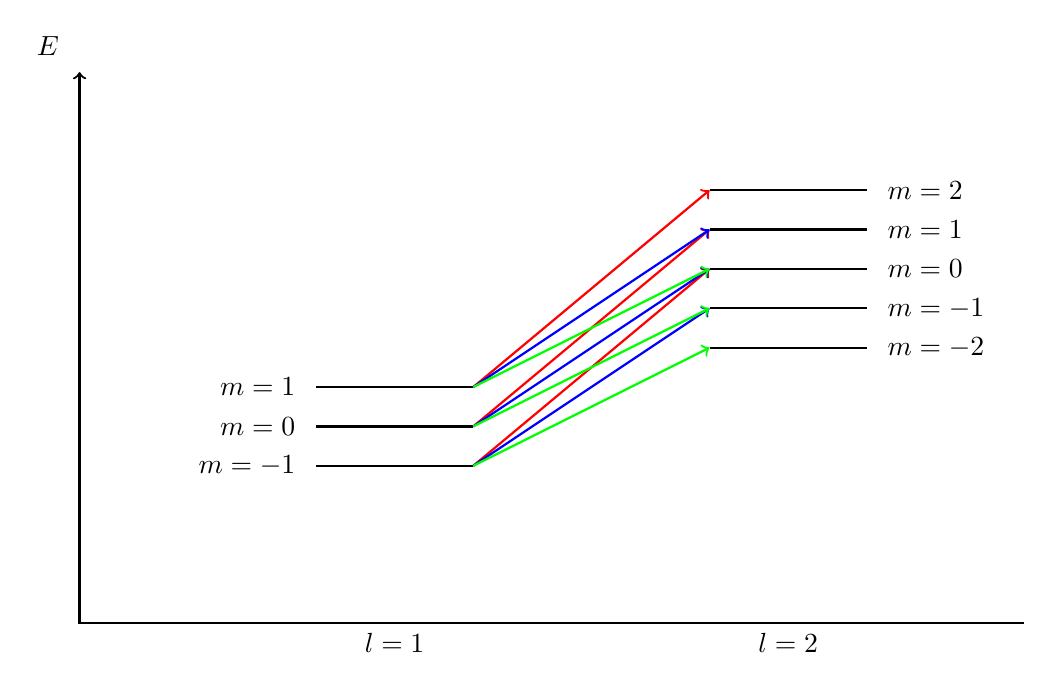
\begin{tikzpicture}
        \draw[->, thick] (9,-2) to (-3,-2) to (-3,5) node[label=150:$E$] {};

        \draw[thick] (0,0) node[label=180:{$m=-1$}] {} -- (2,0) coordinate (l1m-1);
        \draw[thick] (0,.5) node[label=180:{$m=0$}] {} -- (2,.5) coordinate (l1m0);
        \draw[thick] (0,1) node[label=180:{$m=1$}] {} -- (2,1) coordinate (l1m1);
        \node[below] (l1) at (1,-2) {$l=1$};

        \draw[thick] (5,1.5) coordinate (l2m-2) -- (7,1.5)node[label=0:{$m=-2$}] {} ;
        \draw[thick] (5,2) coordinate (l2m-1) -- (7,2)node[label=0:{$m=-1$}] {} ;
        \draw[thick] (5,2.5) coordinate (l2m0) -- (7,2.5)node[label=0:{$m=0$}] {} ;
        \draw[thick] (5,3) coordinate (l2m1) -- (7,3)node[label=0:{$m=1$}] {} ;
        \draw[thick] (5,3.5) coordinate (l2m2) -- (7,3.5)node[label=0:{$m=2$}] {} ;
        \node[below] (l2) at (6,-2) {$l=2$};
        \draw[red, ->, thick] (l1m-1) to (l2m0);
        \draw[red, ->, thick] (l1m0) to (l2m1);
        \draw[red, ->, thick] (l1m1) to (l2m2);
        \draw[blue, ->, thick] (l1m-1) to (l2m-1);
        \draw[blue, ->, thick] (l1m0) to (l2m0);
        \draw[blue, ->, thick] (l1m1) to (l2m1);
        \draw[green, ->, thick] (l1m-1) to (l2m-2);
        \draw[green, ->, thick] (l1m0) to (l2m-1);
        \draw[green, ->, thick] (l1m1) to (l2m0);
    \end{tikzpicture}

    \caption{%
        Mögliche Übergänge zwischen $l=2$ und $l=1$.
    }
    \label{fig:Übergänge}
\end{figure}

\section{Natürliche Linienbreite und Linienverbreiterung}

In Abschnitt \ref{ssec:Niveau} ist die Rede von Linien, die durch diskrete
Energieniveaus hervorgerufen werden. Demnach müsste eine Linie nur genau aus
einer Wellenlänge bestehen. Dies kann jedoch in der Realität nicht beobachtet
werden, neben der Natürlichen Linienbreite, die durch eine endliche
Anregungsdauer hervorgerufen wird findet eine Linienverbreiterung statt.

Hat ein strahlendes Material eine Temperatur $T>\SI{0}{\kelvin}$, bewegen sich
die Teilchen ungeordnet in alle Richtungen. Je nach dem wie groß die Komponente
der Geschwindigkeit in Beobachtungsrichtung ist, findet eine entsprechend
starke Dopplerverschiebung der Wellenlänge statt. Die eigentlich scharfe Linie
wird so zu einer Verteilung von nah aneinander liegenden Wellenlängen. Sie
verbreitert sich also.

Die Frequenzverbreiterung ist gegeben durch
\parencite{chemgapedia/spektrallinien/dopplerverbreiterung}:
\[
    \Deltaup \nu_{1/2} = \num{7.16e-7} \nu_0
    \sqrt{\frac{T / \si\kelvin}{m / \si\atomicmassunit}}.
\]

Die Wellenlängenverbreiterung erhalten wir durch Gauß'sche
Fehlerfortpflanzung:
\[
    \Deltaup \lambda = \frac{c}{\nu_0^2} \Deltaup \nu.
\]

Für eine Temperatur von \SI{1000}{\kelvin} und einem Atomgewicht von \SI{<<
m_cd >>}{\atomicmassunit} \parencite[Umschlag]{meschede-gerthsen_24} erhalten
wir so eine Linienverbreiterung von \SI{<< doppler_width_nu >>}{\hertz} oder
\SI{<< doppler_width_lambda >>}{\pico\meter}.

\section{Fabry-Pérot-Etalon}

Das Fabry-Pérot-Etalon besteht aus einen planparallelen lichtdurchlässigen
Material mit Brechungsindex $n>1$, dessen Oberflächen zum Beispiel durch
Aufdampfen von Silber eine hohe Reflexivität haben.

Trifft ein monochromatischer Lichtstrahl mit Wellenlänge $\lambda$ unter dem
Winkel $\alpha$ auf das Etalon, wird er gebrochen und in diesem sehr häufig
reflektiert (siehe Abbildung~\ref{fig:Etalon}). Bei jeder Reflektion gelangt
ein kleiner Teil der Intensität aus dem Etalon und verlässt diesen wieder unter
dem Winkel $\alpha$. Ist der Gangunterschied zwischen zwei Teilstrahlen nun ein
vielfaches der Wellenlänge findet konstruktive Interferenz statt, gilt dies
nicht, heben sich die Teilstrahlen gegenseitig auf. Die Bedingung für
konstruktive Interferenz lässt sich aus Abbildung~\ref{fig:Etalon} geometrisch
herleiten. Sie lautet
\begin{align*}
    k\lambda &= 2d\cos\del{\beta} - 2d\tan\del{\beta}\cos\del{1-\alpha}.
    \intertext{%
        Über den Brechungsindex erhält man einen Ausdruck für den Winkel
        $\beta$:
    }
    \beta &= \arcsin\del{\frac{\sin{\alpha}}n}
    \intertext{%
        Dadurch ergibt sich für die Interferenzbedingung:
    }
    k\lambda &=
\end{align*}
\begin{figure}
    \centering
    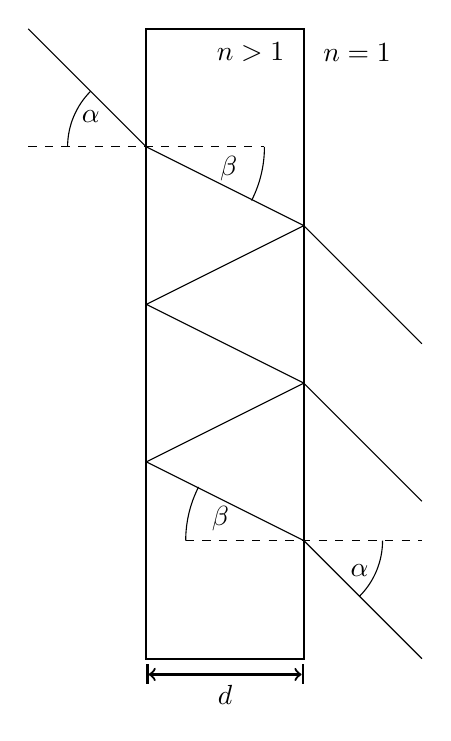
\begin{tikzpicture}
        % Etalon
        \draw[thick] (-1,-4.5) rectangle (1,3.5);
        % Dicke
        \draw[thick, |<->|] (-1,-4.7) to node[below] {$d$} (1,-4.7);
        % Brechungsindizes
        \node[label=180:{$n>1$}, label=0:{$n=1$}] at (1,3.2) {};
        % Lot
        \draw[dashed]
        (-2.5,2.) -- (0.5,2.)
        (-0.5,-3.) -- (2.5,-3.);
        % Strahlengang
        \draw
        (-2.5,3.5) -- (-1,2.)
        -- (1,1) coordinate (a)
        -- (2.5,-.5)
        (a) -- (-1,0)
        -- (1,-1) coordinate (b)
        -- (2.5,-2.5)
        (b) -- (-1,-2)
        -- (1,-3)
        -- (2.5,-4.5);
        % Winkel
        \draw
        (-2.0,2.) arc (180:135:1.0cm) node[label=270:$\alpha$]{}
        (0.5,2.) arc (0:-27:1.5cm) node[label=115:{$\beta$}]{}
        (-0.5,-3.) arc (180:153:1.5cm) node[label=290:$\beta$]{}
        (2,-3.) arc (0:-45:1.0cm) node[label=90:{$\alpha$}]{};
    \end{tikzpicture}
    \caption{%
        Strahlengang im Fabry-Pérot-Etalon
    }
    \label{fig:Etalon}
\end{figure}

\section{Polarisationsfilter und $\frac{\lambda}4$-Plättchen}

Ein Polarisationsfilter oder Linear-Polarisator ist ein optisches Bauteil, mit
dem Licht mit mehreren Polarisationsrichtungen gefiltert werden kann.
Anschaulich wird dabei eine einfallende Welle in zwei Komponenten zerlegt, eine
parallel und eine senkrecht zur Polarisationsrichtung des Filters polarisierte.
Durchgelassen wird nur die parallele Komponente, das Licht ist nun linear
polarisiert.

Ein $\frac\lambda4$-Plättchen ist ein optisches Element, mit dem eine zirkulär
polarisierte Welle in eine linear polarisierte umgewandelt werden kann und
umgekehrt. Es besteht aus einem Material, welches in verschiedene Richtungen
unterschiedliche Brechungsindizes hat. Rechnerisch wird die Welle in zwei
orthogonale Komponenten aufgespalten, welche das Material unterschiedlich
schnell durchdringen. Dabei kommt es zu einer Verschiebung, die, bei richtiger
Wahl der Dicke, genau ein viertel der Wellenlänge entspricht.

\section{Hall-Sonde}

Durch den Hall-Effekt wird in einem stromdurchflossenen Leiterstück, welches
von einem Magnetfeld durchsetzt wird, eine Spannung, die Hall-Spannung erzeugt.
Diese Spannung ist proportional zur Senkrecht auf dem Strom stehenden
Komponente des Magnetfeldes:
\[
    B = \frac{U}{R_\text{HS}I}
\]
Die Hall-Konstante hängt dabei vom Material und von der Geometrie des
Leiterstücks ab. Ist sie bekannt, kann bei eingestelltem Strom die Spannung
vermessen und so das Magnetfeld bestimmt werden.

\section{Frank-Hertz-Versuch}

\subsection{Aufbau und Funktionsweise}
\label{ssec:Aufbau_FH}

\begin{figure}
    \centering
    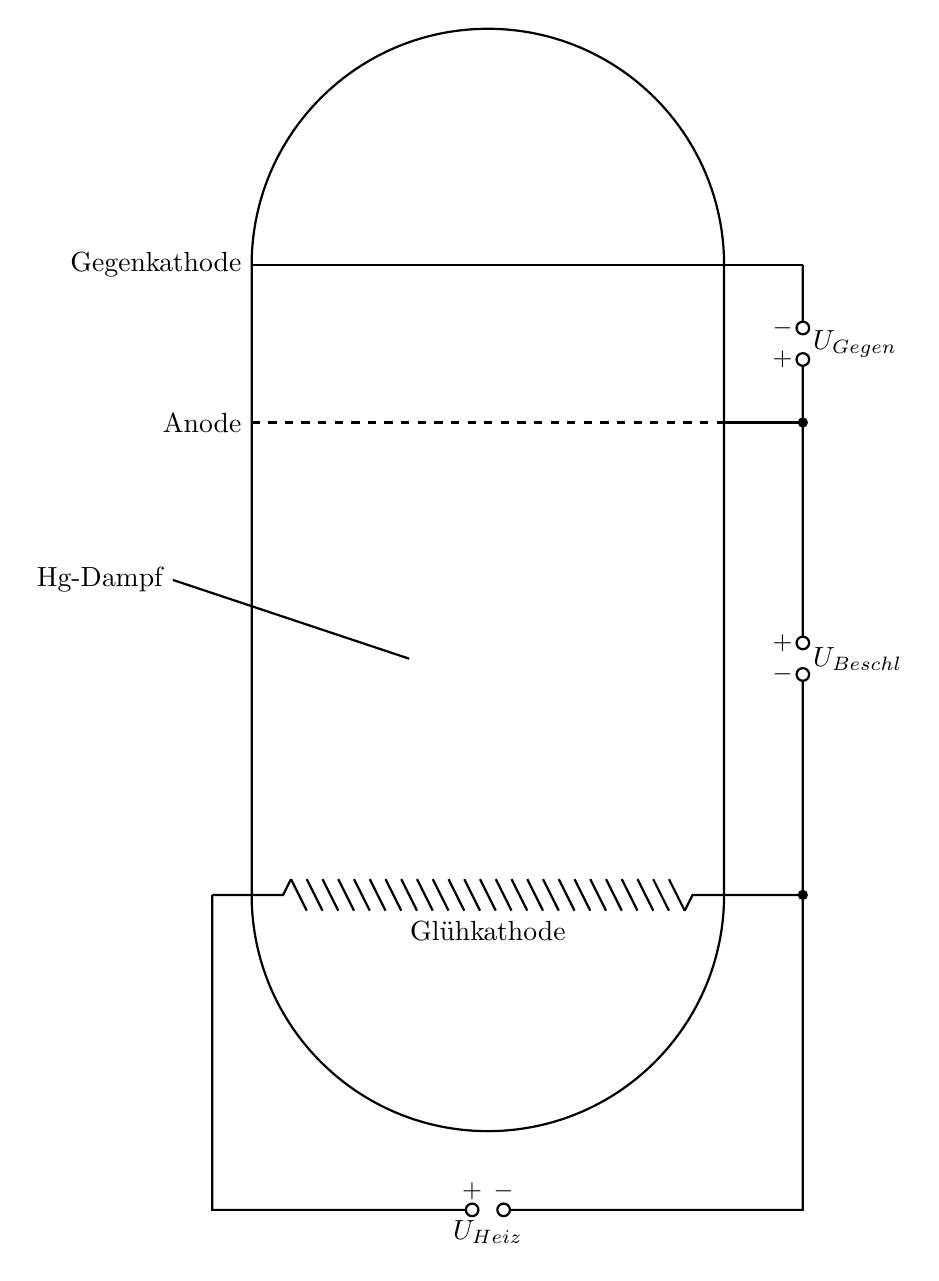
\begin{tikzpicture}[thick]
        % Röhre
        \draw
            (-3,4) -- (-3,-4)
            arc(180:360:3)
            -- (3,4)
            arc(0:180:3);
        % Gegenkathode
        \draw (-3,4) node[left] {Gegenkathode} -- (4,4);
        % Anode
        \draw[dashed](-3,2) node[left] {Anode}-- (3,2);
        \draw (3,2) -- (4,2);
        % Glühkathode
        \draw (-3.5,-4) -- (-2.6,-4) -- (-2.5, -3.8);
        \foreach \x in {-2.5, -2.3, ..., 2.3}
            \draw (\x,-3.8) -- (\x+0.2,-4.2);
        \draw (2.5,-4.2) -- (2.6,-4) -- (4,-4);
        % Verschaltung
        \draw
            (-3.5,-4) -- (-3.5, -8) -- (-0.28, -8)
            (-.2,-8) circle(0.08) node[above] {\small{$+$}}
            (.2,-8) circle(0.08) node[above] {\small{$-$}}
            (0.28, -8) -- (4, -8) -- (4, -4) -- (4, -1.28)
            (4, -1.2) circle(0.08) node[left] {\small{$-$}}
            (4, -0.8) circle(0.08) node[left] {\small{$+$}}
            (4, -0.72) -- (4, 2.72)
            (4, 2.8) circle(0.08) node[left] {\small{$+$}}
            (4, 3.2) circle(0.08) node[left] {\small{$-$}}
            (4, 3.28) -- (4,4)
        ;
        \draw[fill]
            (4,-4) circle(0.05)
            (4,2) circle(0.05);
        % weitere Beschriftungen
        \node[below] at (0,-8) {$U_\text{Heiz}$};
        \node[right] at (4,-1) {$U_\text{Beschl}$};
        \node[right] at (4, 3) {$U_\text{Gegen}$};
        \node[below] at (0,-4.2) {Glühkathode};
        % Füllung
        \draw
        (-4,0) node[left] {Hg-Dampf} -- (-1,-1);
    \end{tikzpicture}
    \caption{%
        Aufbau des Frank-Hertz-Versuchs.
    }
    \label{fig:Aufbau_FH}
\end{figure}

Der Aufbau des Frank-Hertz-Versuchs ist in Abbildung~\ref{fig:Aufbau_FH} zu
sehen.

\subsection{Termschema von Quecksilber}

\begin{figure}[htbp]
    \centering
    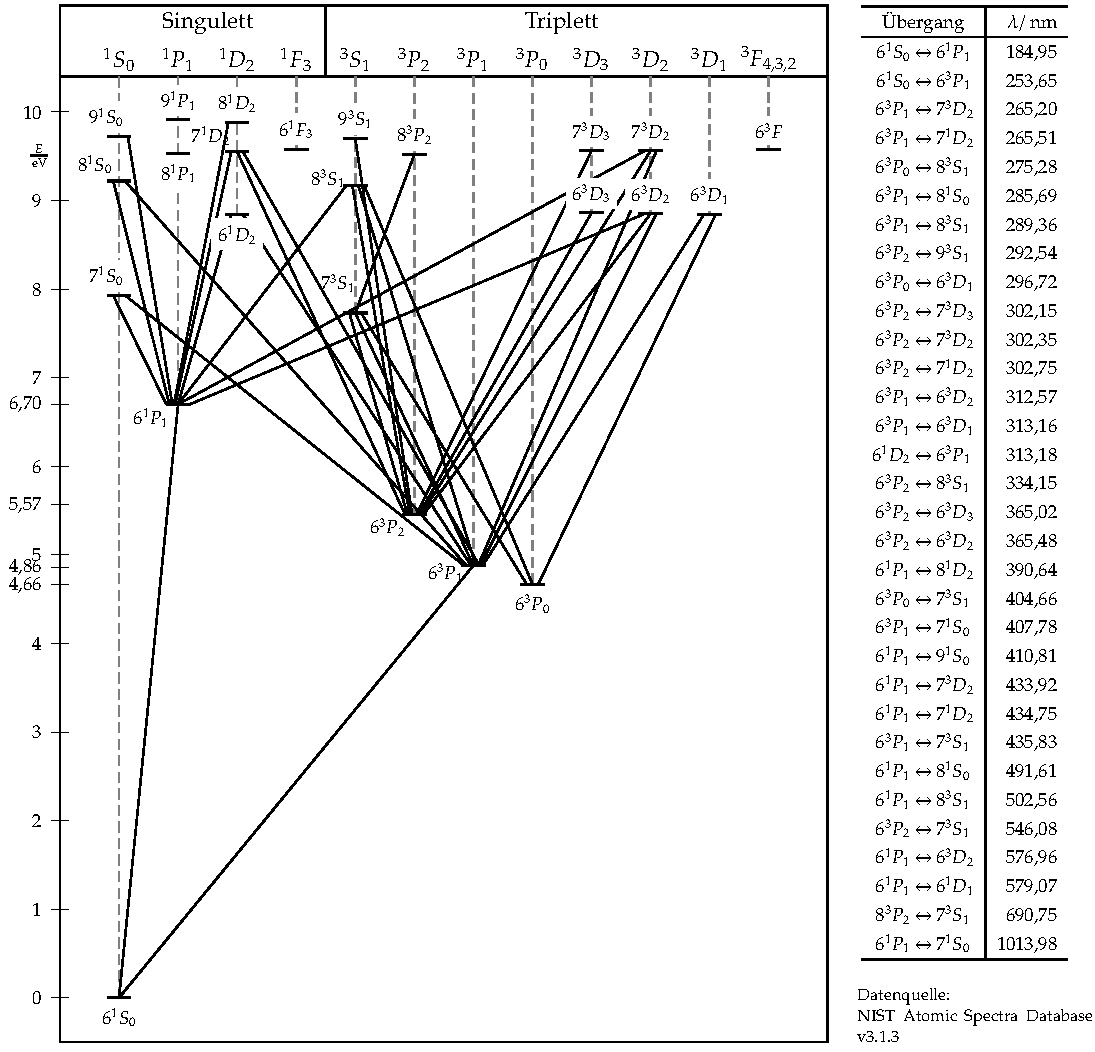
\includegraphics[width=\linewidth]{../termschema_quecksilber.pdf}
    \caption{%
        Termschema von Quecksilber. Lizenziert unter \ccbyncsa.
        \parencite{Kraehling/Termschema_Quecksilber}.
    }
    \label{fig:Termschema}
\end{figure}

\chapter{Zeeman-Effekt}

\section{Qualitative Beobachtung der Aufspaltung}

\subsection{Transversale Konfiguration}

Zuerst betrachten wir die Aufspaltung durch das Okular und fertigen qualitative
Skizzen an. Die beobachtete Linie ist rot, daher haben wir dies als Hauptfarbe
genommen. Um die (roten) Aufspaltungen unterscheiden zu können, sind diese in
der Skizze blau.

Ohne Magnetfeld erhalten wir konzentrische Kreise
(Abbildung~\ref{fig:Skizze-1}). Hier sind die drei Energieniveaus entartet, da
kein externe magnetische Flussdichte anliegt. Jeder Ring ist ein
Interferenzmaximum des Etalons und hat nichts mit der Zeeman-Aufspaltung zu
tun.

\begin{figure}[htbp]
    \centering
    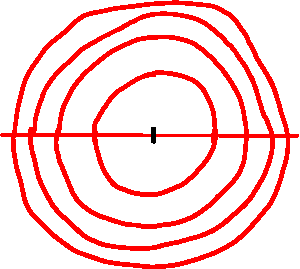
\includegraphics{../Skizze-1.pdf}
    \caption{%
        Transversal, ohne Magnetfeld.
    }
    \label{fig:Skizze-1}
\end{figure}

Wir erhöhen das Magnetfeld, bis wir die aufgespaltenen Ringe gut unterscheiden
können (Abbildung~\ref{fig:Skizze-2}). Der Strom, bei der die Linien zu
unterscheiden sind, ist \SI{<< I_crit_trans >>}{\ampere}. Die Aufspaltung der
Ringe kommt durch die Zeeman-Aufspaltung der Energieniveaus. 

\begin{figure}[htbp]
    \centering
    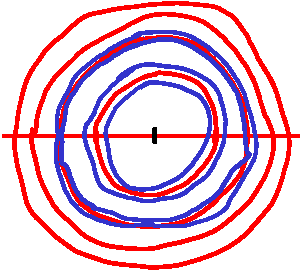
\includegraphics{../Skizze-2.pdf}
    \caption{%
        Transversal, mit Magnetfeld.
    }
    \label{fig:Skizze-2}
\end{figure}

Als nächstes betrachten wir die Polarisation, siehe
Abbildung~\ref{fig:Skizze-3} und \ref{fig:Skizze-4}.

\begin{figure}[htbp]
    \centering
    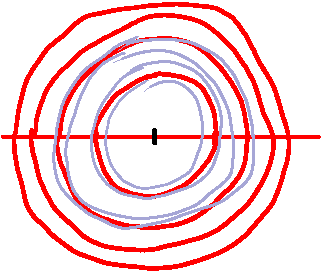
\includegraphics{../Skizze-3.pdf}
    \caption{%
        Transversal, mit Magnetfeld und \SI{90}{\degree} Linearpolarisator.
    }
    \label{fig:Skizze-3}
\end{figure}

\begin{figure}[htbp]
    \centering
    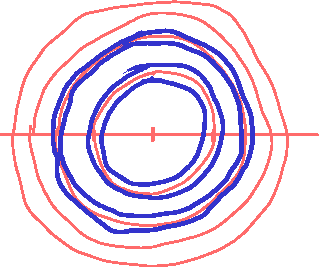
\includegraphics{../Skizze-4.pdf}
    \caption{%
        Transversal, mit Magnetfeld und \SI{0}{\degree} Linearpolarisator.
    }
    \label{fig:Skizze-4}
\end{figure}

\subsection{Longitudinale Konfiguration}

Ohne Magnetfeld beobachten wir das gleiche wie in transversaler Konfiguration,
siehe Abbildung~\ref{fig:Skizze-5}.

\begin{figure}[htbp]
    \centering
    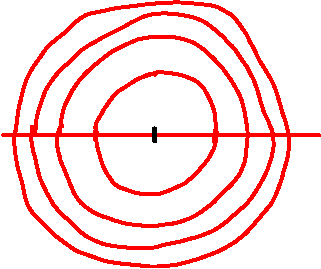
\includegraphics{../Skizze-5.pdf}
    \caption{%
        Longitudinal, ohne Magnetfeld.
    }
    \label{fig:Skizze-5}
\end{figure}

Nun fahren wir wieder den Magnetstrom so hoch, dass wir die Linien trennen
können (Abbildung~\ref{fig:Skizze-6}). In longitudinaler Konfiguration ist der
kritische Strom \SI{<< I_crit_long >>}{\ampere}. Die longitudinalen Linien sind
deutlich dunkler. Außerdem gibt es nur noch zwei Linien, keine mittlere Linie
mehr. Dies liegt daran, dass in longitudinaler Richtung durch das Photon
positiver oder negativer Drehimpuls weggetragen werden muss, da sich die
$z$-Komponente des Drehimpulses des ausstrahlenden Elektrons ändert. Daher gibt
es nur zwei Möglichkeiten: positive und negative Helizität, also zirkulare
Polarisation links und rechts herum.

\begin{figure}[htbp]
    \centering
    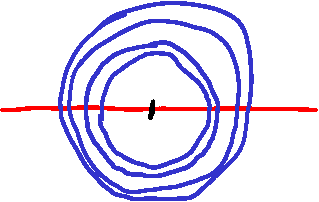
\includegraphics{../Skizze-6.pdf}
    \caption{%
        Longitudinal, mit Magnetfeld.
    }
    \label{fig:Skizze-6}
\end{figure}

Mit einer $\lambda/4$-Platte konvertieren wir die zirkulare Polarisation in
Lineare und können so die Helizität unterscheiden (Abbildung~\ref{fig:Skizze-7}
und \ref{fig:Skizze-8}). So können wir zeigen, dass die beiden Ringe
tatsächlich den Übergängen mit $\Deltaup m_l = \pm 1$ entsprechen.

\begin{figure}[htbp]
    \centering
    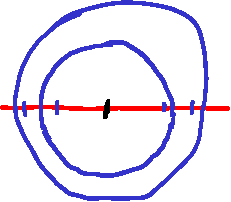
\includegraphics{../Skizze-7.pdf}
    \caption{%
        Longitudinal, mit Magnetfeld, \SI{0}{\degree} $\lambda/4$-Platte und
        \SI{-45}{\degree} Linearpolarisator.
    }
    \label{fig:Skizze-7}
\end{figure}

\begin{figure}[htbp]
    \centering
    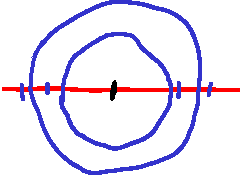
\includegraphics{../Skizze-8.pdf}
    \caption{%
        Longitudinal, mit Magnetfeld, \SI{0}{\degree} $\lambda/4$-Platte und
        \SI{+45}{\degree} Linearpolarisator.
    }
    \label{fig:Skizze-8}
\end{figure}

\section{Magnetfeldkalibrierung}

Wir fahren den Strom durch und lassen die Cassy-Software Strom und Induktion
registrieren.

An die Messdaten passen wir ein Polynom dritter Ordnung, $B(I) = a + bI + cI^2
+ dI^3$, an. Als Parameter erhalten wir durch die Anpassung:
\begin{align*}
    a &= \SI{<< mfk_a >>}{\milli\tesla} \\
    b &= \SI{<< mfk_b >>}{\milli\tesla\per\ampere} \\
    c &= \SI{<< mfk_c >>}{\milli\tesla\per\ampere\squared} \\
    d &= \SI{<< mfk_d >>}{\micro\tesla\per\ampere\cubed}
\end{align*}

Daten und Anpassung sind in Abbildung~\ref{fig:Magnetfeldkalibrierung}
dargestellt. Da die Anpassung gut passt, haben wir keine vierte Ordnung
hinzugefügt.

\begin{figure}[htbp]
    \centering
    \includegraphics[width=\linewidth]{Magnetfeldkalibrierung.pdf}
    \caption{%
        Anpassung der Daten aus der Hallsonde gegen den Strom.
    }
    \label{fig:Magnetfeldkalibrierung}
\end{figure}

Im weiteren Verlauf der Auswertung werden wir diese Funktion benutzen, um
Ströme in Magnetfelder umzurechnen.

\section{Messung der Aufspaltung}

Die Messwerte für alle Flussdichten sind in Abbildung~\ref{fig:Alles}
dargestellt.

\begin{figure}[htbp]
    \centering
    \includegraphics[width=\linewidth]{Alles.pdf}
    \caption{%
        Zusammenstellung aller Messdaten aus diesem Versuchsteil.
    }
    \label{fig:Alles}
\end{figure}

Wir rechnen die gemessenen Winkel in Wellenlängen um. Dazu benutzen wir als
Wellenlänge für Cadmium \SI{<< lambda_cd >>}{\meter}
\parencite{NIST/Strong_Lines_of_Cadmium} \footnote{%
    Diese Quelle scheint eine Zusammenstellung zu sein. Die besagte Linie wird
    dort wiederum mit „K. Burns and K. B. Adams, J. Opt. Soc. Am. 46, 94
    (1956).“ zitiert.
}. Diese ist genau auch die, die der Filter durchlässt.

Die Anzahl der Maxima, die das Etalon erzeugt, ist durch
\[
    m_\text{max} = \frac{2nd}{\lambda}
\]
gegeben. Mit den gegebenen Werten erhalten wir \num{<< m_max >>} Maxima. Der
innerste Ring hat die Ordnung $m_\text{max} - 1$. Wir rechnen nun mit
\[
    \lambda = \frac{2 n d \cos(\alpha)}{m_\text{max} - 1}
\]
die Winkel in Wellenlängen um. Dabei stimmt natürlich nur das erste Maximum. Wir
wählen das erste Maximum auf der Seite der negativen Winkel aus. Dieser ist in
Abbildung~\ref{fig:Zoom} dargestellt.

\begin{figure}[htbp]
    \centering
    \includegraphics[width=\linewidth]{Zoom.pdf}
    \caption{%
        Ausschnittsvergrößerung des ersten richtigen Maximums auf der linken
        Seite von Abbildung~\ref{fig:Alles}. Die Farben haben die gleiche
        Bedeutung. Die Winkel sind hier schon in Wellenlängen umgerechnet.
    }
    \label{fig:Zoom}
\end{figure}

Für jede Flussdichte passen wir eine Summe aus drei Gaußkurven sowie einem
konstanten Untergrundsignal an die Messdaten an. Unsere Gaußkurve ist wie folgt
definiert:
\begin{equation}
    \label{eq:gauss}
    \mathop{\text{Gauß}} (x; \mu, \sigma, a)
    := a \exp\del{- \frac12 \del{\frac{x-\mu}{\sigma}}^2}
\end{equation}

Aus der Anpassung erhalten wir die Schwerpunkte der Maxima, siehe
Tabelle~\ref{tab:Peakschwerpunkte}. Die Daten und ihre Anpassungen sind in den
Abbildungen \ref{fig:Fit-<< I_list[0] >>} bis \ref{fig:Fit-<< I_list[-1] >>}
gezeigt. Die Anpassung konvergiert aufgrund der 10 Freiheitsgrade nicht
zuverlässig. Wir mussten die Startwerte sehr nah an den optimalen Werten
wählen, um überhaupt eine Konvergenz zu erhalten. Die Einträge in der
Fehlermatrix sind jedoch um mehrere Größenordnungen größer als die Parameter
selbst. Da die Ergebnisse jedoch brauchbar aussehen, nehmen wir die
Standardabweichung aus den einzelnen Gaußkurven als Fehler für den Schwerpunkt.
Fehlerangaben gehen implizit von Gaußverteilung aus, also ist dies in diesem
Fall genau richtig.

%< for I in I_list: >%
\begin{figure}[htbp]
    \centering
    \includegraphics[width=.8\linewidth]{Fit-<< I >>.pdf}
    \caption{%
        Daten und Anpassung für \SI{<< I >>}{\ampere}, entsprechend \SI{<<
        B_dict[I] >>}{\centi\tesla}.
    }
    \label{fig:Fit-<< I >>}
\end{figure}
%< endfor >%

\begin{table}[htbp]
    \centering
    \begin{tabular}{SSSSS}
        {$I / \si{\ampere}$}
        & {$B / \si{\centi\tesla}$}
        & {$\lambda_- / \si{\nano\meter}$}
        & {$\lambda_0 / \si{\nano\meter}$}
        & {$\lambda_+ / \si{\nano\meter}$} 
        \\
        \midrule
        %<- for row in fit_tabelle: ->%
        << ' & '.join(row) >> \\
        %<- endfor ->%
    \end{tabular}
    \caption{%
        Schwerpunkte der Maxima.
    }
    \label{tab:Peakschwerpunkte}
\end{table}

Die Schwerpunkte aus Tabelle~\ref{tab:Peakschwerpunkte} rechnen wir in
Energiedifferenzen aus. Dabei ist die Verschiebung der Wellenlänge:
\[
    \Deltaup \lambda = \frac{\lambda_+ - \lambda_-}2.
\]

Daraus bestimmt sich die Energiedifferenz
\[
    \Deltaup E = \frac{hc\Deltaup\lambda}{\lambda_0^2}
\]
für jede Flussdichte. Diese Daten sind in
Tabelle~\ref{tab:Energieaufspaltungen} zusammengetragen.

\begin{table}[htbp]
    \centering
    \begin{tabular}{SSS}
        {$B / \si{\centi\tesla}$}
        & {$\Deltaup \lambda / \si{\pico\meter}$} 
        & {$\Deltaup E / \SI{e-25}{\joule}$} 
        \\
        \midrule
        %<- for row in energieaufspaltung_tabelle: ->%
        << ' & '.join(row) >> \\
        %<- endfor ->%
    \end{tabular}
    \caption{%
        Energieaufspaltungen
    }
    \label{tab:Energieaufspaltungen}
\end{table}

Wir tragen die Aufspaltung gegen die Flussdichte auf
(Abbildung~\ref{fig:Energieaufspaltung}) und passen eine Ursprungsgerade an.
Die Steigung ist das Bohr'sche Magneton:
\[
    \mu_\text B = \SI{<< bohr_magneton >>}{\joule\per\tesla}.
\]

\begin{figure}[htbp]
    \centering
    \includegraphics[width=\linewidth]{Energieaufspaltung.pdf}
    \caption{%
        Energieaufspaltung
    }
    \label{fig:Energieaufspaltung}
\end{figure}

\section{Auflösungsvermögen und Finesse}

\subsection{Theoretische Werte}

Für die Finesse erhalten wir:
\[
    \mathcal F_\text{theo.} = \frac{\piup \sqrt r}{r-1} = \num{<< finesse_theoretisch >>}.
\]

Und das Auflösungsvermögen erhalten wir mit dem freien Spektralbereich
$\Deltaup \nu = c / (2nd)$. Wir errechnen $\Deltaup \lambda = c \Deltaup \nu /
\nu^2$ mit der Frequenz $\nu$ der Cadmiumlinie. Somit erhalten wir:
\[
    N_\text{theo.} = \num{<< N_theoretisch >>}.
\]

\subsection{Werte aus qualitativer Messung}

Wir hatten die Aufspaltung ab einem Magnetstrom von \SI{<< I_crit_trans
>>}{\ampere} und \SI{<< I_crit_long >>}{\ampere} in der transversalen bzw\@.
longitudinalen Konfiguration erkennen können. Dies entspricht Magnetfeldern von
\SI{<< B_crit_trans >>}{\centi\tesla} bzw\@. \SI{<< B_crit_long >>}{\centi\tesla}.

Mit unserem errechneten Bohr'schen Magneton können wir daraus nun eine
Energiedifferenz
\[
    \Deltaup E = \mu_\text B B(I)
\]
bestimmen, aus der wir dann wiederum eine Wellenlängendifferenz errechnen:
\[
    \lambda = \frac1\nu = \frac{hc}{E}
    \implies
    \Deltaup \lambda
    = \frac{hc}{E^2} \Deltaup E
    = \frac{\lambda^2}{hc} \Deltaup E.
\]

Daraus können wir dann das Auflösungsvermögen berechnen:
\[
    N = \frac{\lambda}{\Deltaup \lambda}
    = \frac{hc}{\lambda \Deltaup E}.
\]

Somit erhalten wir $N_\text{trans.} = \num{<< N_trans >>}$ und $N_\text{long.}
= \num{<< N_long >>}$.

Finesse \fehlt

\subsection{Werte aus CCD Messung}

\fehlt

\subsection{Vergleich}

\fehlt

\section{Diskussion}

Der Literaturwert für das Bohr'sche Magneton ist:
\parencite{wikipedia/Bohr_Magneton} \parencite[Umschlag]{meschede-gerthsen_24}
\[
    \mu_\text B = \SI{9.274e-24}{\joule\per\tesla}.
\]

Unser Wert von \SI{<< bohr_magneton >>}{\joule\per\tesla} liegt um einen Faktor
4 zu hoch.

\chapter{Frank-Hertz-Versuch}

\section{Durchführung}

\section{Auswertung}

Unsere Messdaten sind für einen ersten Überblick in
Abbildung~\ref{fig:FH_Rohdaten} dargestellt.

\begin{figure}[htbp]
    \centering
    \includegraphics[width=\linewidth]{FH_Rohdaten.pdf}
    \caption{%
        Rohdaten zum Franck-Hertz-Versuch.
    }
    \label{fig:FH_Rohdaten}
\end{figure}

\subsection{Bestimmung der Energiedifferenz}

An jede der Kurve passen wir folgende Überlagerung aus fünf äquidistanten
Gaußfunktionen \eqref{eq:gauss} mit unterschiedlicher Amplitude und einer
Ursprungsgeraden an:
\begin{multline*}
    U_\text A (U_\text B; U_{\text B, \text{min}}, U_\text{Abstand}, U_\text{Breite}, \{a_i\}, m)
    = \\
    \sum_{i=1}^5 \mathop{\text{Gauß}} (U_\text B; U_{\text B, \text{min}} + i
    U_\text{Abstand}, U_\text{Breite}, a_i)
    +
    m U_\text B.
\end{multline*}

Wir benutzen Gaußkurven, da wir an den Schwerpunkten der Maxima interessiert
sind. In den Graphen ist zu sehen, dass die Maxima tatsächlich annähernd
gaußförmig sind. Den linearen Teil haben wir hinzugefügt, da die Minima
annähernd auf einer Geraden liegen. Bei hohen Beschleunigungsspannungen liegen
die Minima etwas höher, so dass hier eventuell noch ein quadratischer Term
benutzt werden kann. Jedoch passen die Kurven gut und konvergieren ausreichend
schnell. Daher lassen wir diesen Teil weg.

Aufgrund des Plateaus benutzen wir nur die Messwerte bis zu einer
Beschleunigungsspannung von \SI{<< upper_limit >>}{\volt}.

%< for s in fh_sets: >%
\begin{figure}[htbp]
    \centering
    \includegraphics[width=0.8\linewidth]{<< s.filename >>}
    \caption{%
        $T = \SI{<< s.T >>}{\kelvin}$,
        $U_\text G = \SI{<< s.U_G >>}{\volt}$,
        $U_\text{Abstand} = \SI{<< s.abstand >>}{\volt}$,
        $U_\text{Breite} = \SI{<< s.breite >>}{\volt}$.
    }
    \label{fig:}
\end{figure}
%< endfor >%

Die beiden interessanten Parameter sind $U_\text{Abstand}$ und
$U_\text{Breite}$. Bei der Anpassung wird das erste Maximum trotz entsprechend
gewählter Startwerte nicht berücksichtigt. Dies ist jedoch kein Problem, da der
Abstand der weiteren Maxima richtig herauskommt. Die errechneten Parameter sind
in Tabelle~\ref{tab:fh-fit1} zusammengetragen.

\begin{table}[htbp]
    \centering
    \begin{tabular}{SSSS}
        {$T / \si\kelvin$}
        & {$\Deltaup U_G / \si\volt$}
        & {$U_{\text{Abstand}} / \si\volt$}
        & {$U_{\text{Breite}} / \si\volt$}
        \\
        \midrule
        %< for s in fh_sets: >%
        << s.T >> & << s.U_G >> & << s.abstand >> & << s.breite >> \\
        %< endfor >%
    \end{tabular}
    \caption{%
        Zusammenstellung der Anpassungsparameter.
    }
    \label{tab:fh-fit1}
\end{table}

\FloatBarrier
\subsection{Energiedifferenzen}

Wir rechnen die Spannungsdifferenzen in Wellenzahlunterschiede um, wobei wir
die Variante mit $k = \lambda^{-1}$ (anstelle von $k = 2\piup\lambda^{-1}$)
benutzen:
\[
    k = \frac{U_{\text{Abstand}} e}{h c}
    \eqnsep
    \lambda = \frac 1k.
\]
Die erhaltenen Wellenzahlen und -längen sind in Tabelle~\ref{tab:fh-k_lambda}.

\begin{table}[htbp]
    \centering
    \begin{tabular}{SSS}
        {$U_{\text{Abstand}} / \si\volt$}
        & {$k / \si{\per\centi\meter}$}
        & {$\lambda / \si{\nano\meter}$}
        \\
        \midrule
        %< for s in fh_sets: >%
        << s.abstand >> & << s.k >> & << s.lambda >> \\
        %< endfor >%
    \end{tabular}
    \caption{%
        Wellenzahl und -länge der Übergänge.
    }
    \label{tab:fh-k_lambda}
\end{table}

Der einzige Übergang, der aus dem Termschema in Abbildung~\ref{fig:Termschema}
in Frage kommt, ist der $\mathrm{6{}^1S_0 \to 6{}^3P_1}$ mit
\SI{253.65}{\nano\meter}. Dieser Übergang hat auch einen maximalen
Wirkungsquerschnitt (siehe \cite[Abbildung~P401.5]{physik412-Anleitung}) bei
Elektronenenergien von \SI{5}{\electronvolt}, dies entspricht ebenfalls unseren
Überlegungen.

\subsection{Abhängigkeit des Anodenstroms}

Bei ganzen Vielfachen der Anregungsenergie gibt es keinen scharfen Einbruch, da
trotzdem einige Elektronen die Anode erreichen. Dies können sie aus einem der
folgenden Gründen:

Die angeregten Zustände haben eine gewisse Lebensdauer. Innerhalb dieser Zeit
kann ein Atom kein weiteres Energiequant von \SI{5}{\electronvolt} aufnehmen.
Das Elektron fliegt ungestört weiter.

Das Quecksilber ist recht dünn (einige \si{\deka\pascal}, siehe
Abbildung~\ref{fig:Dampfdruckkurve}), so dass die freie Weglänge der
Quecksilberatome \SIrange{0.1}{100}{\micro\meter} beträgt
\parencite{wikipedia/Mittlere_freie_Weglaenge}. Daher kann es auch sein, dass
ein Elektron, wenn es die richtige kinetische Energie hat, kein Quecksilberatom
trifft. Je höher die Spannung ist, desto schmaler wird der Raumbereich, in dem
das Elektron die richtige Energie hat.

In Abbildung~\ref{fig:FH_Rohdaten} sind alle Messdaten zusammengestellt. Den
höchsten Anodenstrom haben wir für die niedrigste Temperatur, also für den
niedrigsten Druck erhalten. Im Graph ist zu sehen, dass der lineare Teil dort
auch am stärksten ist. Dies interpretieren wir so, dass die Elektronen dort
häufig keinen Stoßpartner finden. Aus diesem Grund sind auch die Maxima höher.

Die letzten vier Kurven in Abbildung~\ref{fig:FH_Rohdaten} sind bei gleicher
Temperatur, jedoch mit unterschiedlichen Gegenspannungen aufgenommen. Die
türkise und die lila Kurve, also für Gegenspannungen von \SIlist{1;2}{\volt}
unterscheiden sich in den Maxima kaum, in den Minima jedoch recht deutlich.

Die Gleichheit in den Maxima liegt daran, dass ein Maximum genau dann entsteht,
wenn der letzte Elektronenstoß eine halbe Beschleunigungsstrecke (für einen
weiteren Stoß) von der Anode entfernt liegt. Die Elektronen haben so die
maximale kinetische Energie und können mit \SI{2.5}{\electronvolt} gegen die
Gegenspannung laufen.

Bei einer Gegenspannung von \SIlist{3;4}{\volt} (gelb und schwarz) ist die
halbe Stoßenergie von \SI{2.5}{\electronvolt} jedoch nicht mehr genug. Daher
werden jetzt auch im Maximum weniger Elektronen durchgelassen, der Anodenstrom
sinkt.

Die höhere Gegenspannung verhindert ebenfalls, das Elektronen, die gerade
gestoßen sind, noch die Anode erreichen. Dies führt dann dazu, dass die Minima
bei höherer Gegenspannung tiefer liegen.

\subsection{Dampfdruck}

Innerhalb des recht kleinen Temperaturintervalles von
\SIrange{150}{165}{\celsius} ist die Dampfdruckkurve von Quecksilber in
Abbildung~\ref{fig:Dampfdruckkurve} dargestellt. Die relative Schwankung, die
Differenz der Extremwerte durch den Mittelwert, beträgt \num{<< ddk_schwankung
>>}. Dies ist schon relativ viel für einen kleinen Temperaturbereich. Die Atome
dürfen nicht zu dicht sein, damit die Elektronen auch wirklich beschleunigt
werden können, ohne zu oft zu stoßen. Jedoch müssen auch genug Atome vorhanden
sein, damit die Elektronen nicht ohne Widerstand durch das dünne Gas kommen. In
diesem Fall wären die Minima nicht deutlich ausgeprägt.

\begin{figure}[htbp]
    \centering
    \includegraphics[width=\linewidth]{Dampfdruckkurve.pdf}
    \caption{%
        Dampfdruck in Abhängigkeit von der Temperatur.
    }
    \label{fig:Dampfdruckkurve}
\end{figure}

\section{Diskussion}

\printbibliography

\end{document}

% vim: et spell spelllang=de tw=79
